\documentclass{article}
%\url{https://tex.stackexchange.com/q/534491/86}
\usepackage{tikz}
\usetikzlibrary{decorations.markings,knots}

\tikzset{% 
    arrowat/.style={%
        postaction={decorate,decoration={
                markings,
                mark=at position #1 with {\arrow[xshift=2pt]{>}}}}
    }
}
\begin{document}

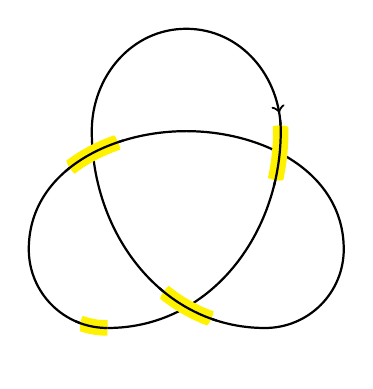
\begin{tikzpicture}
\begin{knot} [
  consider self intersections,
  ignore endpoint intersections=false,
  clip width=7,
  flip crossing=3,
  background colour=yellow,
  only when rendering/.style={
    arrowat=0.8
  }
]
    \strand [thick] (0,0)
    to [out=180, in=270] (-1,1)
    to [out=90, in=180] (1,2.5)
    to [out=0, in=90] (3,1)
    to [out=270, in=0] (2,0)
    to [out=180, in=270] (-0.2,2.5)
    to [out=90, in=180] (1,3.8)
    to [out=0, in=90] (2.2,2.5)
    to [out=270, in=0] (0,0);
\end{knot}
\end{tikzpicture}

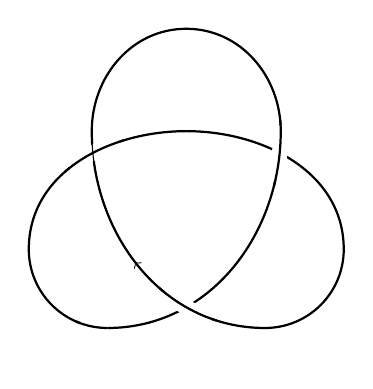
\begin{tikzpicture}
\begin{knot} [
  consider self intersections,
  ignore endpoint intersections=false,
  clip width=7,
  flip crossing=3,
]
    \strand [thick, spath/save global=strand]
(0,0)
    to [out=180, in=270] (-1,1)
    to [out=90, in=180] (1,2.5)
    to [out=0, in=90] (3,1)
    to [out=270, in=0] (2,0)
    to [out=180, in=270] (-0.2,2.5)
    to [out=90, in=180] (1,3.8)
    to [out=0, in=90] (2.2,2.5)
    to [out=270, in=0] (0,0)
    ;
\end{knot}
\draw[spath/restore=strand, arrowat=0.5];
\end{tikzpicture}

\end{document}
